\documentclass[12pt, aspectratio=169]{beamer}

\input{../header}
\usepackage{booktabs}

\title{Correlation Analysis}
\author{Md. Aminul Islam Shazid}
\date{}


\begin{document}
    {
        \setbeamertemplate{footline}{}
        \addtocounter{framenumber}{-2}

        \begin{frame}
            \titlepage
        \end{frame}

        \begin{frame}{Outline}
            \vfill
            \tableofcontents[subsectionstyle=hide]
            \vfill
        \end{frame}
    }


    \section{Introduction}


    \begin{frame}{What is Correlation?}
        \begin{itemize}
            \item In many real-world situations, two or more variables tend to
                move \textbf{together}
            \begin{itemize}
                \item Height and weight of individuals
                \item Study hours and exam scores
                \item Number of family members and monthly food expenditure
                \item Temperature and ice cream sales
            \end{itemize}
            \item \textbf{Correlation analysis} is a statistical technique used to
                measure the \textbf{degree} and \textbf{direction} of the linear
                relationship between two quantitative variables
            \item The primary objectives are to determine:
            \begin{itemize}
                \item \textbf{Strength:} how closely are the variables related?
                \item \textbf{Direction:} do they increase together, or does one
                    decrease as the other increases?
            \end{itemize}
            \item \textbf{Important:} correlation only measures \emph{linear}
                association; it does not imply cause and effect
        \end{itemize}
    \end{frame}


    \begin{frame}{Motivating Example}
        A researcher records the \textbf{number of family members} ($X$) and \textbf{monthly expenditure on food} in thousand taka ($Y$) for 7 families:

        \begin{columns}
            \begin{column}{0.45\textwidth}
                \begin{center}
                    \vspace{-0.5em}
                    \small
                    \begin{tabular}{cc}
                        \hline
                        \textbf{$x$} & \textbf{$y$} \\
                        \hline
                        2  & 5  \\
                        3  & 7  \\
                        6  & 11 \\
                        4  & 8  \\
                        7  & 13 \\
                        3  & 6  \\
                        6  & 12 \\
                        \hline
                    \end{tabular}
                \end{center}

                \vspace{-0.5em}

                Intuitively, as family size increases, food expenditure should also increase. But \emph{how strong} is this relationship?
            \end{column}
            \begin{column}{0.55\textwidth}
                \begin{center}
                    \vspace{-1.5em}
                    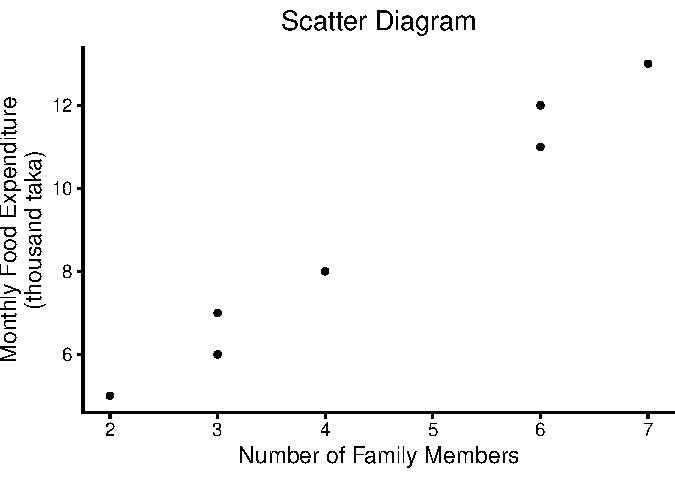
\includegraphics[width=\textwidth]{plots/corr-motivating-scatter.pdf}
                \end{center}
            \end{column}
        \end{columns}
    \end{frame}


    \section{Types of Correlation}


    \begin{frame}{Types of Correlation}
        \begin{columns}
            \begin{column}{0.5\textwidth}
                \begin{center}
                    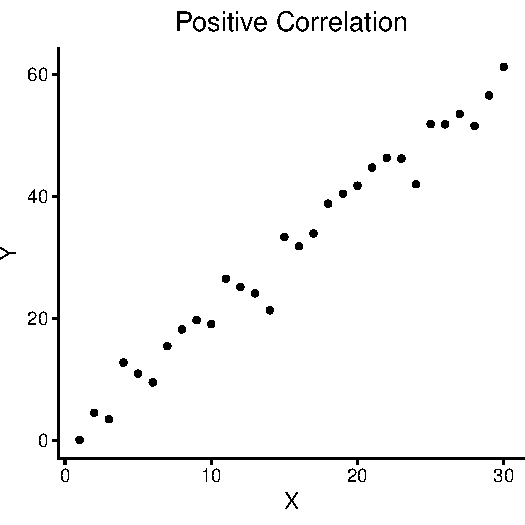
\includegraphics[width=\textwidth]{plots/corr-positive.pdf}
                \end{center}
            \end{column}
            \begin{column}{0.5\textwidth}
                \begin{center}
                    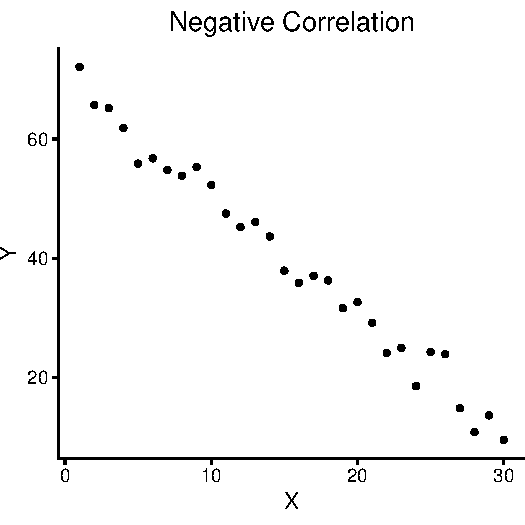
\includegraphics[width=\textwidth]{plots/corr-negative.pdf}
                \end{center}
            \end{column}
        \end{columns}
    \end{frame}


    \begin{frame}{Types of Correlation (cont.)}
        \begin{columns}
            \begin{column}{0.5\textwidth}
                \begin{center}
                    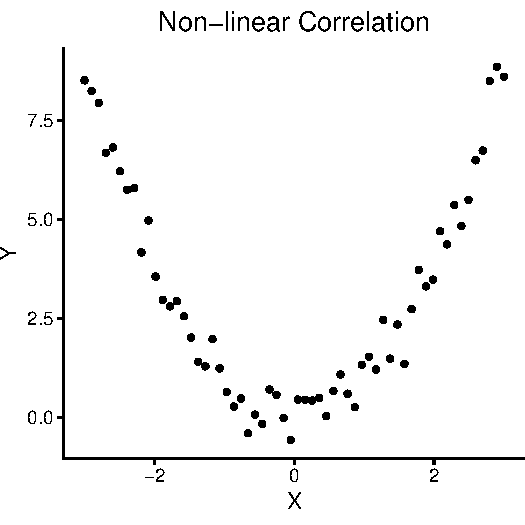
\includegraphics[width=\textwidth]{plots/corr-nonlinear.pdf}
                \end{center}
            \end{column}
            \begin{column}{0.5\textwidth}
                \begin{center}
                    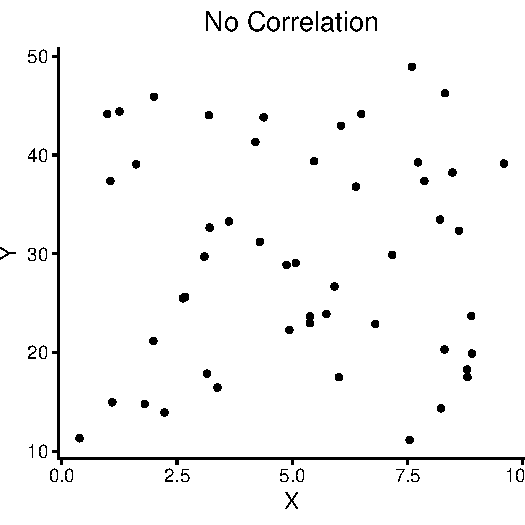
\includegraphics[width=\textwidth]{plots/corr-none.pdf}
                \end{center}
            \end{column}
        \end{columns}
        % R code to generate non-linear correlation plot:
        % library(ggplot2); set.seed(3)
        % x <- seq(-3, 3, length.out = 60)
        % df <- data.frame(x = x, y = x^2 + rnorm(60, sd = 0.5))
        % ggplot(df, aes(x, y)) +
        %   geom_point(size = 2) +
        %   labs(title = "Non-linear Correlation", x = "X", y = "Y") +
        %   theme_classic() +
        %   theme(plot.title = element_text(hjust = 0.5))
        % ggsave("plots/corr-nonlinear.pdf", width = 3.5, height = 2.8)
        %
        % R code to generate no correlation plot:
        % library(ggplot2); set.seed(4)
        % df <- data.frame(x = runif(50, 0, 10), y = runif(50, 10, 50))
        % ggplot(df, aes(x, y)) +
        %   geom_point(size = 2) +
        %   labs(title = "No Correlation", x = "X", y = "Y") +
        %   theme_classic() +
        %   theme(plot.title = element_text(hjust = 0.5))
        % ggsave("plots/corr-none.pdf", width = 3.5, height = 2.8)
    \end{frame}


    \begin{frame}{Types of Correlation --- Summary}
        \begin{itemize}
            \item \textbf{Positive correlation:} as $X$ increases, $Y$ tends to
                increase as well
            \begin{itemize}
                \item Example: family size and food expenditure; height and weight
            \end{itemize}
            \item \textbf{Negative correlation:} as $X$ increases, $Y$ tends to
                decrease
            \begin{itemize}
                \item Example: price of a product and its demand; hours of TV
                    watched and exam scores
            \end{itemize}
            \item \textbf{No linear correlation:} no consistent linear pattern
                between $X$ and $Y$
            \begin{itemize}
                \item Example: shoe size and intelligence
            \end{itemize}
            \item \textbf{Non-linear (curvilinear) correlation:} $X$ and $Y$ are
                related, but not in a straight-line fashion
            \begin{itemize}
                \item Example: age and athletic performance
                \item \textbf{Note}: Pearson's $r$ \emph{cannot} capture this ---
                    it would report a value near zero even though a strong
                    relationship exists
            \end{itemize}
        \end{itemize}
    \end{frame}


    \section{Pearson's Correlation Coefficient}


    \begin{frame}{Pearson's Correlation Coefficient}
        \begin{itemize}
            \item The most widely used measure of linear association between two
                quantitative variables
            \item Denoted $r$ for the \textbf{sample} and $\rho$ (rho) for the
                \textbf{population}
            \item Formula:
            \[
                r = \frac{\text{cov}(X,Y)}{\sqrt{v(X)}\,\sqrt{v(Y)}}
                  = \frac{\displaystyle\sum (x_i-\bar{x})(y_i-\bar{y})}
                         {\sqrt{\displaystyle\sum(x_i-\bar{x})^2}\;
                          \sqrt{\displaystyle\sum(y_i-\bar{y})^2}}
            \]
            \item Computationally convenient form:
            \[
                r = \frac{n\sum xy - \sum x\sum y}
                         {\sqrt{n\sum x^2 - \left(\sum x\right)^2}\;
                          \sqrt{n\sum y^2 - \left(\sum y\right)^2}}
            \]
            \item $X$ and $Y$ are two quantitative variables; $n$ is the number
                of observations
        \end{itemize}
    \end{frame}


    \begin{frame}{Interpretation of $r$}
        \begin{itemize}
            \item $r > 0$: positive linear relationship
            \item $r < 0$: negative linear relationship
            \item $r = 0$: no \emph{linear} relationship
        \end{itemize}

        \vspace{0.4em}

        \begin{center}
            \small
            \begin{tabular}{ccc}
                \toprule
                \textbf{Value of $r$} & \textbf{Direction} & \textbf{Strength} \\
                \midrule
                $r = 1$ & Positive & Perfect \\
                $0.50 \leqslant r < 1$ & Positive & Strong \\
                $0 < r < 0.50$ & Positive & Weak \\
                $r = 0$ & --- & No linear correlation \\
                $-0.50 < r < 0$ & Negative & Weak \\
                $-1 < r \leqslant -0.50$ & Negative & Strong \\
                $r = -1$ & Negative & Perfect \\
                \bottomrule
            \end{tabular}
        \end{center}

        \vspace{0.3em}

        \begin{itemize}
            \item The range of $r$ is always $-1 \leqslant r \leqslant 1$
            % \item $|r| = 1$ indicates a \textbf{perfect} linear relationship --- all points lie exactly on a straight line
        \end{itemize}
    \end{frame}


    \begin{frame}{Assumptions}
        \begin{itemize}
            \item Both $X$ and $Y$ are measured on an \textbf{interval or ratio}
                scale
            \item The pair $(X, Y)$ follows a \textbf{bivariate normal
                distribution}
            \item The relationship between the variables is \textbf{linear}
            \item The sample is of \textbf{adequate size} to assume normality
        \end{itemize}
    \end{frame}


    \begin{frame}{Example --- Computation Table}
        \begin{center}
            \small
            \begin{tabular}{ccccc}
                \hline
                $x$ & $y$ & $x^2$ & $y^2$ & $xy$ \\
                \hline
                2 & 5  & 4  & 25  & 10 \\
                3 & 7  & 9  & 49  & 21 \\
                6 & 11 & 36 & 121 & 66 \\
                4 & 8  & 16 & 64  & 32 \\
                7 & 13 & 49 & 169 & 91 \\
                3 & 6  & 9  & 36  & 18 \\
                6 & 12 & 36 & 144 & 72 \\
                \hline
                $\sum x = 31$ & $\sum y = 62$ & $\sum x^2 = 159$ &
                $\sum y^2 = 608$ & $\sum xy = 310$ \\
                \hline
            \end{tabular}
        \end{center}

        \vspace{0.5em}

        \begin{align*}
            r = \frac{n\sum xy - \sum x\sum y}
                     {\sqrt{n\sum x^2 - \left(\sum x\right)^2}\;
                      \sqrt{n\sum y^2 - \left(\sum y\right)^2}}
              &= \frac{7 \times 310 - 31 \times 62}
                     {\sqrt{7 \times 159 - 31^2}\;\sqrt{7 \times 608 - 62^2}} \\
              &= 0.991
        \end{align*}
    \end{frame}


    \begin{frame}{Example --- Interpretation}
        \begin{columns}
            \begin{column}{0.5\textwidth}
                Here, \(0.991\). This indicates a \textbf{very strong positive} linear relationship
                between the number of family members and monthly food expenditure.
                As family size increases, food expenditure also tends to increase,
                and the two variables move very closely together.

                \vspace{0.5em}

                Since $r = 0.991 \approx 1$, the data points lie very close to a
                straight line, indicating an almost perfect linear association.
            \end{column}
            \begin{column}{0.5\textwidth}
                \begin{center}
                    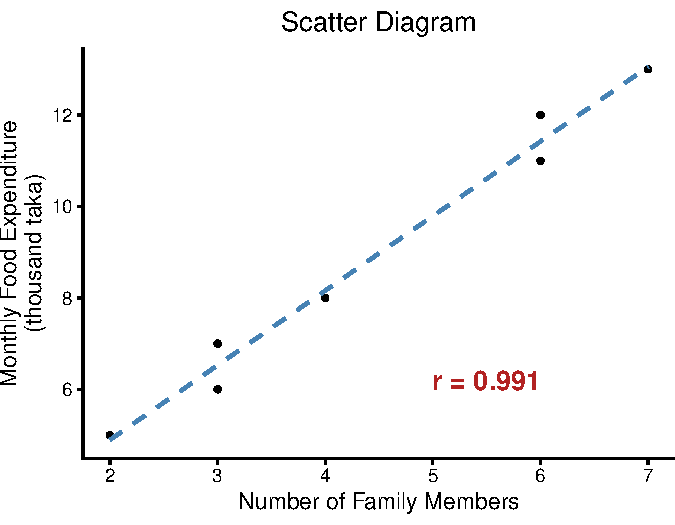
\includegraphics[width=\textwidth]{plots/corr-scatter-annotated.pdf}
                \end{center}
            \end{column}
        \end{columns}
    \end{frame}


    \section{Properties of Correlation}


    \begin{frame}{Properties of the Correlation Coefficient}
        \begin{itemize}
            \item $r$ \textbf{always measures linear relationships} only; a value
                near zero does not rule out a strong non-linear relationship
            \item $r = 0$ means no \emph{linear} relationship --- $X$ and $Y$ may
                still be strongly related in a non-linear way
            \item $r_{xy} = r_{yx}$: the correlation coefficient is
                \textbf{symmetric} --- the correlation of $X$ with $Y$ equals the
                correlation of $Y$ with $X$
            \item $r$ is \textbf{dimensionless} --- it carries no units of
                measurement, making it comparable across different studies and
                variables
            \item $r$ is \textbf{not affected} by a change of origin or scale
                (i.e.\ adding a constant or multiplying by a positive constant
                does not change $r$)
            \item $r^2$ (the \textbf{coefficient of determination}) gives the
                proportion of the variation in $Y$ that can be explained by its
                linear relationship with $X$
        \end{itemize}
    \end{frame}


    \section{Correlation is Not Causation}


    \begin{frame}{Correlation Does Not Imply Causation}
        \begin{itemize}
            \item A high $|r|$ tells us that $X$ and $Y$ tend to move together
                --- it says \textbf{nothing} about \emph{why} they do so
            \item Three possible explanations for a strong correlation:
            \begin{itemize}
                \item \textbf{Direct causation:} $X$ causes $Y$
                    (e.g.\ more rainfall $\to$ more crop yield)
                \item \textbf{Reverse causation:} $Y$ actually causes $X$
                \item \textbf{Confounding (spurious correlation):} a third
                    variable $Z$ drives both $X$ and $Y$, creating an apparent
                    but misleading relationship between them
            \end{itemize}
            \item \textbf{Classic example of spurious correlation:}
                Countries with higher chocolate consumption per capita tend to
                produce more Nobel laureates.
                Clearly, eating chocolate does not cause Nobel prizes ---
                national wealth is a confounding variable driving both
            \item \textbf{Rule of thumb:} correlation is a useful first step,
                but establishing causation requires controlled experiments or
                careful causal reasoning --- not just a high $r$
        \end{itemize}
    \end{frame}


    \section{Test for the Correlation Coefficient}


    \begin{frame}{Why Test the Correlation Coefficient?}
        \begin{itemize}
            \item The computed value of $r$ is based on \textbf{sample data}
            \item Even if the true population correlation $\rho = 0$, a random
                sample will almost never give exactly $r = 0$ due to
                \textbf{sampling variability}
            \item For example, with a small sample of $n = 7$, even a moderate
                $r$ could have arisen purely by chance
            \item We therefore need a \textbf{formal hypothesis test} to decide
                whether the observed $r$ is large enough to conclude that a genuine
                linear relationship exists in the \textbf{population}
            \item This test answers the question:
            \begin{center}
                \emph{``Is the observed sample correlation $r$ statistically
                significant, or is it just sampling noise?''}
            \end{center}
        \end{itemize}
    \end{frame}


    \begin{frame}{Hypotheses}
        \begin{itemize}
            \item Let $\rho$ denote the \textbf{population} correlation coefficient
            \item $H_0: \rho = 0$ represents the claim that there is
                \textbf{no linear relationship} between $X$ and $Y$ in the population
            \item \textbf{Two-tailed} (test for any linear association):
            \[
                H_0: \rho = 0 \quad \text{vs} \quad H_A: \rho \neq 0
            \]
            \item \textbf{Right-tailed} (test for positive linear association):
            \[
                H_0: \rho = 0 \quad \text{vs} \quad H_A: \rho > 0
            \]
            \item \textbf{Left-tailed} (test for negative linear association):
            \[
                H_0: \rho = 0 \quad \text{vs} \quad H_A: \rho < 0
            \]
            \item We \textbf{do not} conclude that $\rho = 0$ if we fail to
                reject $H_0$; we simply lack sufficient evidence to claim
                otherwise
        \end{itemize}
    \end{frame}


    \begin{frame}{Test Statistic}
        \begin{itemize}
            \item Under $H_0: \rho = 0$, the test statistic is:
            \[
                t_{\text{cal}} = \frac{r\,\sqrt{n-2}}{\sqrt{1-r^2}} \sim t_{n-2}
            \]
            where $r$ is the sample correlation coefficient and $n$ is the
            sample size
            \item The test statistic follows a \textbf{$t$-distribution with
                $n - 2$ degrees of freedom} under $H_0$
            \item \textbf{Intuition:}
            \begin{itemize}
                \item A large $|r|$ (strong linear relationship) produces a large
                    $|t_{\text{cal}}|$, pushing the statistic into the rejection
                    region
                \item A small $|r|$ (weak relationship) produces a small
                    $|t_{\text{cal}}|$, consistent with $H_0$
                \item For a fixed $r$, a \emph{larger} $n$ produces a larger
                    $|t_{\text{cal}}|$ --- with enough data, even a weak
                    correlation can become statistically significant
            \end{itemize}
        \end{itemize}
    \end{frame}


    \begin{frame}{General Testing Procedure}
        \begin{itemize}
            \item State $H_0$ and $H_A$; identify whether the test is one-tailed
                or two-tailed
            \item Choose the level of significance $\alpha$
            \item Compute the sample correlation coefficient $r$ and the test
                statistic:
            \[
                t_{\text{cal}} = \frac{r\,\sqrt{n-2}}{\sqrt{1-r^2}}
            \]
            \item Determine the critical value $t_{\alpha/2,\;n-2}$ (two-tailed)
                or $t_{\alpha,\;n-2}$ (one-tailed) from the $t$-table
            \item \textbf{Decision rule:}
            \begin{itemize}
                \item Two-tailed: reject $H_0$ if
                    $|t_{\text{cal}}| > t_{\alpha/2,\;n-2}$
                \item Right-tailed: reject $H_0$ if
                    $t_{\text{cal}} > t_{\alpha,\;n-2}$
                \item Left-tailed: reject $H_0$ if
                    $t_{\text{cal}} < -t_{\alpha,\;n-2}$
            \end{itemize}
            \item State a conclusion in the context of the problem
        \end{itemize}
    \end{frame}


    \begin{frame}{Example --- Hypotheses and Test Statistic}
        \textbf{Question:} Using the family members and food expenditure data,
        test at $\alpha = 0.05$ whether there is a significant linear relationship
        between number of family members and monthly food expenditure.

        \vspace{0.8em}

        Let $\rho =$ population correlation coefficient between $X$ and $Y$.

        \[
            H_0: \rho = 0 \quad \text{vs} \quad H_A: \rho \neq 0
        \]

        \vspace{0.5em}

        From the earlier computation: $r = 0.991$, $n = 7$.

        \vspace{0.3em}

        \textbf{Test statistic:}
        \[
            t_{\text{cal}}
            = \frac{r\,\sqrt{n-2}}{\sqrt{1-r^2}}
            = \frac{0.991 \times \sqrt{5}}{\sqrt{1 - 0.991^2}}
            = \frac{0.991 \times 2.236}{\sqrt{0.0182}}
            = \frac{2.216}{0.134}
            \approx 16.56
        \]
    \end{frame}


    \begin{frame}{Example --- Solution}
        \begin{columns}
            \begin{column}{0.55\textwidth}
                \textbf{Degrees of freedom:} $n - 2 = 5$

                \vspace{0.4em}

                \textbf{Critical value:} $t_{0.025,\;5} = 2.571$

                \vspace{0.4em}

                \textbf{Decision:} Since $|t_{\text{cal}}| = 16.56 > 2.571$,
                we \textbf{reject} $H_0$ at 5\% level of significance.

                \vspace{0.4em}

                \textbf{P-value:}
                $p = 2\,P(t_5 \geqslant 16.56) \approx 0.000$

                Since $p < \alpha = 0.05$, we reject $H_0$.

                \vspace{0.4em}

                \textbf{Conclusion:} There is very strong evidence of a significant
                positive linear relationship between number of family members and
                monthly food expenditure in the population.
            \end{column}
            \begin{column}{0.45\textwidth}
                \begin{center}
                    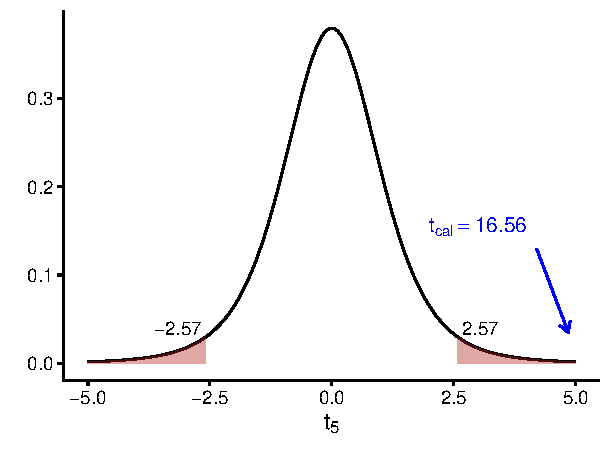
\includegraphics[width=\textwidth]{plots/corr-t-test.pdf}
                \end{center}
            \end{column}
        \end{columns}
    \end{frame}


    % \section{Assignment}


    % \begin{frame}{Assignment Question}
    %     \textbf{Q8.} The purpose of a study by Brown and Persley was to characterize
    %     acute hepatitis~A in patients more than 40 years old. They performed a
    %     retrospective chart review of 14~subjects who were diagnosed with acute
    %     hepatitis~A, but were not hospitalized. Of interest was the relationship
    %     between age (years) and bilirubin levels (mg/dl). The following data
    %     were collected.

    %     \vspace{0.3em}

    %     \emph{(Add the last two digits of your student ID to each $y$ value:
    %     new $y$ = original $y$ + last two digits of ID)}

    %     \vspace{0.5em}

    %     \begin{itemize}
    %         \item[(a)] Draw a scatter diagram of the data.
    %         \item[(b)] Calculate Pearson's correlation coefficient between age
    %             and amount of bilirubin. Interpret your result.
    %         \item[(c)] Test whether the population correlation coefficient between
    %             age and bilirubin level is significantly different from zero.
    %             Use $\alpha = 0.05$.
    %     \end{itemize}
    % \end{frame}


    \section*{Thank you.}

\end{document}